\chapter{Modèles nucléaires}

\section{Introduction}
L'équation de Schrödinger $H\Psi=E\Psi$ d'un noyau ne peut pas être résolue exactement pour $A>4$. Le problème
est le terme potentiel qui - bien qu'il paraît inoffensif - cache une double somme
\begin{equation}
H=\sum_{i=1}^AT_i+\sum_{i>j=1}^A V_{ij}
\end{equation}
où $T_i=\vec{p_i^2}/(2m_N)$ est l'énergie cinétique du nucléon $i$ et $V_{ij}$ l'interaction entre les nucléons
$i$ et $j$.\\

En plus de n'être pas résolvable analytiquement, le potentiel nucléon-nucléon $V_{ij}$ n'est pas exactement 
connu, il existe des forces à 3 corps, 4 corps, \dots ainsi que des effets relativistes difficiles à inclure. Pour
s'en sortir il convient d'utiliser des modèles respectant les principes physiques et reproduisant certaines
propriétés du noyau. Il existe deux classes de modèles
\begin{enumerate}
\item Particules indépendantes : chaque nucléon est pris en compte individuellement
\item Collectifs : le noyau est considéré comme un ensemble
\end{enumerate}


\section{Modèle du gaz de Fermi}
	\begin{wrapfigure}[9]{l}{2.5cm}
	\vspace{-5mm}
	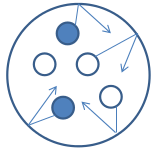
\includegraphics[scale=0.4]{ch8/image1}
	\captionof{figure}{ }
	\end{wrapfigure}
Il s'agit d'un modèle à particules indépendantes
\begin{equation}
\Psi(r_1,r_2,\dots, r_A) = \phi_1(r_1)\phi_2(r_2)\dots\phi_A(r_A)
\end{equation}
Ce modèle considère que les nucléons sont dans une "boîte", dans laquelle ils n'interagissent pas. Ceci est 
décrit par un potentiel de \textit{sphère dure} $V_i(r_i)$
\begin{equation}
V=\sum_{i=1}^A V_i, \qquad\qquad V_i(r_i)=0\ \text{si}\ r\leq a,\qquad\qquad V_i(r_i)=\infty\text{ si }r>a
\end{equation}
Les fonctions individuelles sont celles de particules dans une boîte cubique de côté $a$ 
\begin{equation}
\phi_i(x,y,z) = A\sin(k_xx)\sin(k_yy)\sin(k_zz)
\end{equation}
où $k_xa=n_a\pi,k_ya=n_y\pi$ et $k_za=n_z\pi$. Ce modèle permet d'expliquer certains termes de la formule de 
masse (celui élaboré lors du modèle de la goutte liquide, à savoir le terme de volume et d'asymétrie). 
L'énergie d'individuelle est alors donnée par
\begin{equation}
E(n_x,n_y,n_z) = \frac{a\hbar^2}{2m}(k_x^2+k_y^2+k_z^2) = \frac{\hbar^2k^2}{2m} = \frac{\hbar^2\pi^2}{2ma^2}
(n_x^2+n_y^2+n_z^2)
\end{equation}

\newpage
	\begin{wrapfigure}[11]{r}{5.5cm}
	\vspace{-5mm}
	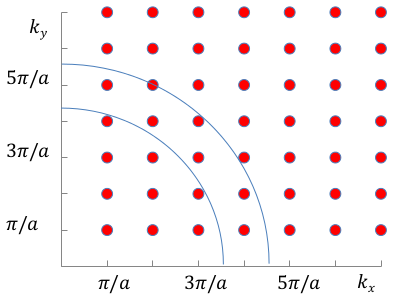
\includegraphics[scale=0.4]{ch8/image2}
	\captionof{figure}{ }
	\end{wrapfigure}
	
Ci-contre, une représentation bidimensionnelle des valeurs d'énergies accessibles pour un nucléon. Chaque état
peut être occupé par maximum quatre nucléons (spin/isospin).Le nombre d'états entre $k$ et $k+dk$ est donné par
\begin{equation}
dn = 4\times 4\pi k^2dk\times\left(\frac{a}{\pi}\right)^3
\end{equation}
où $\pi/a$ est le volume d'une cellule. Dès lors
\begin{equation}
\frac{dn}{dk} = \frac{2}{\pi^2}k^2V
\end{equation}
où $V=a^3$ est le volume du noyau (supposé cubique). Le nombre total de nucléon $A$ doit donc respecter la
relation (l'intégration doit forcément donner le nombre de nucléons)
\begin{equation}
A = \int_0^{k_F} \frac{dn}{dk}dk = \frac{2}{3\pi^2}k_F^2V
\end{equation}
où $\DS k_F = \left(\frac{3\pi^2}{2}\frac{A}{V}\right)^{1/3} = 1.33$ fm$^{-1}$ est le \textbf{nombre d'onde de
Fermi}. Comme la densité $\rho = A/V$ est connue, on peut facilement trouver l'énergie individuelle maximale
dite l'\textbf{énergie de Fermi}
\begin{equation}
\epsilon_F = \frac{\hbar^2k_F^2}{2m_N}=\frac{a\hbar^2}{2m_N}\left(\frac{3\pi^2}{2}\rho\right)^2 \approx
37\ \text{MeV}
\end{equation}


	\begin{wrapfigure}[8]{l}{7.5cm}
	\vspace{-5mm}
	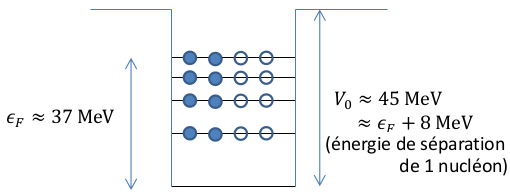
\includegraphics[scale=0.4]{ch8/image3}
	\captionof{figure}{ }
	\end{wrapfigure}
	

Les orbitales sont ainsi remplies jusqu'au niveau de \textsc{Fermi} et il est alors facile, sachant ça, de 
calculer l'énergie totale du noyau en effectuant la somme sur tous les nucléons. 
\begin{equation}
E = \int_0^{k_F} \frac{\hbar^2k^2}{2m_N}dn = \frac{\hbar^2}{2m_N}\frac{2k_F^5}{5\pi^2}V = \frac{3}{5}\epsilon_F
A \approx 22.2\ \text{A}
\end{equation}
On retrouve la forme du terme de volume ($B(Z,A) = a_VA+\dots$). L'énergie est proportionnelle au nombre 
de nucléons ce qui justifie la forme précédemment utilisée.\\



	\begin{wrapfigure}[8]{r}{3cm}
	\vspace{-5mm}
	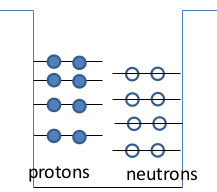
\includegraphics[scale=0.4]{ch8/image4}
	\captionof{figure}{ }
	\end{wrapfigure}
On peut également considérer l'asymétrie neutron-proton en considérant des énergies de \textsc{Fermi} différentes
pour chacune de ces deux espèces\footnote{Si le noyau est asymétrique, l'énergie de liaison diminue.}
\begin{equation}
E_p(Z) = \frac{3}{5}\epsilon_F(p)Z = \frac{\hbar^2}{2m_N}\left(\frac{3\pi^2}{2}\frac{Z}{V}\right)^{2/3}Z
\end{equation}
\begin{equation}
E_n(Z) = \frac{3}{5}\epsilon_F(p)N = \frac{\hbar^2}{2m_N}\left(\frac{3\pi^2}{2}\frac{N}{V}\right)^{2/3}N
\end{equation}
L'énergie d'asymétrie est obtenue en prenant la différence entre deux énergie : l'une qui serait l'énergie 
s'il n'y avait pas de différence entre neutrons et protons et l'autre l'énergie spécifique associée aux 
protons et aux neutrons
\begin{equation}
\Delta E = 2E(A/2)-E(Z)-E(N) = -\frac{1}{3}\epsilon_F\frac{(N-Z)^2}{A}
\end{equation}
On retrouve le terme d'asymétrie dans le modèle de la goutte liquide ($B(A,Z) = \dots - a_a\frac{(N-Z)^2}{A}+
\dots$).\\

\textsc{Conclusions}\\
Ce modèle permet d'expliquer la forme des termes de volume et d'asymétrie (mais pas l'ajustement des 
paramètres). Lorsqu'on s'intéresse aux fonctions d'ondes, dans le modèle de particules indépendantes comme
c'est le cas ici, on obtient un produit de fonctions d'onde individuelles. Celles-ci décrivant des fermions,
il faut que lafonction d'onde soit antisymétrique
\begin{equation}
\Psi(r_1,r_2,\dots, r_A) =\mathcal{A} \phi_1(r_1)\phi_2(r_2)\dots\phi_A(r_A)
\end{equation}
où $A =\sum_{p=1}^{A!} \epsilon_pP_p$ est l'opérateur \textit{anti-symétriseur} avec $P_p$ la permutations de 
$A$ éléments et $\epsilon_p$ le signe de la permutation. Il est possible d'écrire cette fonction d'onde sous
la forme d'un déterminant de \textsc{Slater}.



\section{Modèle rotationnel}
Le \textit{modèle rotationnel} est un modèle collectif associé à la déformation du noyau : les noyaux ne sont
plus sphériques. Découplons la rotation du noyau de sa structure interne
\begin{equation}
H = H_{rot}(\omega) + H_{int}(\vec{r}_i) + H_{conj}
\end{equation}
où le terme conjugué $H_{conj}$ est négligé, où $\omega=(\alpha,\beta,\gamma)$ sont les angles d'\textsc{Euler}
et $\vec{r_i}$ les coordonnées internes du noyau. La fonction d'onde est alors factorisée\footnote{Rappelons
que les noyaux sont ici non sphériques.}
\begin{equation}
\Psi =\varphi(\omega)\Phi(\vec{r_i})
\end{equation}
où $\Phi(\vec{r_i})$ est le fonction d'onde interne, supposée être identique pour tous les états excités (
$\to$ propriétés similaires). Nous verrons un peu plus tard que les $\varphi(\omega)$ sont en réalités les
fonctions de \textsc{Wigner}. \\

Avant toute chose, considérons deux systèmes d'axes : les axes intrinsèques au système (attachés au noyau, 
obtenus par la rotation $\mathcal{R}(\omega)$) et les axes fixes du laboratoire. Sachant que
\begin{equation}
T = \frac{-\hbar^2}{2m}\left( \frac{d^2}{dr^2} + \frac{L^2}{r^2}\right)
\end{equation}
l'hamiltonien de rotation s'écrit
\begin{equation}
H_{rot}(\omega) = \frac{J_1^2}{2\mathcal{J}_1}+\frac{J_1^2}{2\mathcal{J}_2}+\frac{J_3^2}{2\mathcal{J}_3}
\end{equation}
où $J_i$ sont les moments cinétiques par rapport aux axes intrinsèques du noyau et $\mathcal{J}_i$ sont les
moments d'inerties suivant les trois axes : ils sont caractéristiques de la déformation\footnote{Par la suite,
on supposera que deux d'entre-eux sont égaux et différent du troisième : ceci met en évidence la déformation
du noyau, non sphérique.}.\\

Nous savons que $\vec{J}^2$ est un bon nombre quantique
\begin{equation}
\vec{J}^2 : J^2_1+J^2_2+J^2_3=J^2_x+J^2_y+J^2_z
\end{equation}
où les indices $x,y,z$ correspondent à la situation dans le référentiel du laboratoire.\\

Les fonctions propre de $\vec{J}^2$ sont les fonctions de \textsc{Wigner}, $\mathcal{D}_{MK}^J(\alpha,\beta,
\gamma)$ une généralisation des harmoniques sphériques. Notons
\begin{equation}
\begin{array}{lll}
\vec{J}^2\mathcal{D}_{MK}^J(\omega) &= \hbar^2J(J+1)\mathcal{D}_{MK}^J(\omega)\\
J_z\mathcal{D}_{MK}^J(\omega) &= \hbar M\mathcal{D}_{MK}^J(\omega)&\qquad \text{(projection sur l'axe fixe)}\\
J_3\mathcal{D}_{MK}^J(\omega) &= \hbar K\mathcal{D}_{MK}^J(\omega)&\qquad \text{(projection sur l'axe intrinsèque)}
\end{array}
\end{equation}
Le nombre quantique $K$ est un bon nombre quantique approché : $[H_{int}, J_3]\neq0$. Ceci va nosu permettre
de ré-écrire notre fonction d'onde
\begin{equation}
\Psi = \Phi_{int}(\vec r_i)\varphi(\omega)\qquad\text{où } \varphi(\omega) = \mathcal{D}_{MK}^J(\omega)
\end{equation}\ \\

Comme annoncé, nous allons supposer un système axial (la déformation se fait selon le troisième axe)
\begin{equation}
\mathcal{J}_1 = \mathcal{J}_2 = \mathcal{J}
\end{equation}
L'Hamiltonien de rotation devient
\begin{equation}
H_{rot}(\omega) = \frac{J^2}{2\mathcal{J}}+\frac{J_3^2}{2}\left(\frac{1}{\mathcal{J}_3-\frac{1}{\mathcal{J}}}
\right)
\end{equation}
Cet opérateur a comme fonctions propres les fonctions de \textsc{Wigner} $H_{rot}\mathcal{D}_{MK}^J(\omega) =
E_{jk}\mathcal{D}_{MK}^J(\omega)$.\\

\retenir{\textbf{énergies de rotation}
\begin{equation}
E_{JK} = \frac{\hbar^2}{2\mathcal{J}}J(J+1) + E_{0k}
\end{equation}
avec $J \geq |K|$ (inégalités triangulaires).}\ \\

Les fonctions d'ondes associées sont données par
\begin{equation}
\varphi_{MK}^J(\omega) = \left(\frac{2J+1}{8\pi^2}\right)^{1/2}\mathcal{D}_{MK}^J(\omega)
\end{equation}
Celle-ci possède une symétrie de réflexion. Sachant que l'opérateur de réflexion est équivalent à une rotation
de 180$^\circ$, effectuons une telle rotation autour de l'axe principal 2
\begin{equation}
e^{i\pi L_2}\mathcal{D}_{MK}^J(\omega) = (-1)^{J+k}\mathcal{D}_{M-K}^J(\omega)
\end{equation}
Pour la parité, cela équivaut au changement de variable $r\to -r$. La fonction projetée en parité est
\begin{equation}
\varphi_{MK}^{J\pi}(\omega) = \left(\frac{2J+1}{8\pi^2}\right)^{1/2} [\mathcal{D}_{MK}^J(\omega)+
\pi(-1)^{J+k}\mathcal{D}_{M-K}^J(\omega)]
\end{equation}
Dans le cas particulier où $K=0$, $J$ ne peut valoir que $0,2,4,6,\dots$ ou $1,3,5,7,\dots$. Lors de la 
représentation d'un spectre (voir ci-dessous), chaque niveau est de plus en plus éloigné
du précédent. Il s'agit d'une conséquence de $H_{rot}$ (à cause du $J(J+1)$). Chaque bande est dite "\textit{bande
rotationnelles} : le diagramme $E_{JK}$ est linéaire en $J(J+1)$.

\begin{center}
	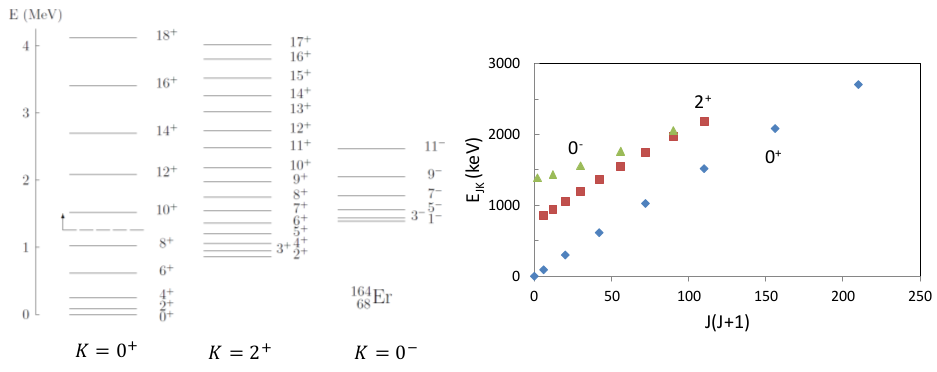
\includegraphics[scale=0.45]{ch8/image5}
	\captionof{figure}{$^{164}_{68}$ Er}
\end{center}

En bleu, cela représenté $K=0^+$. La relation n'est pas parfaitement linéaire mais la tendance l'est fortement. 
On peut contrôler le caractère rotationnel d'une bande grâce à ce phénomène linéaire mais aussi grâce aux
probabilités de transitions qui doivent respecter une certaine forme.



\section{Modèle de potentiel}
Dans la radioactivité $\alpha$, nous avions supposé qu'il existait une particule $\alpha$ proche de la surface
du noyau. Celle-ci peut s'en détacher et interagir avec le noyau sous la forme d'un potentiel : il est temps
de décrire celui-ci. Ce modèle est applicable au noyaux léger (essentiellement la structure $\alpha$). Il est
bien adapté aux collions noyau-noyau et peut être généralisé à trois ou quatre particules.\\

	\begin{wrapfigure}[5]{l}{4.8cm}
	\vspace{-5mm}
	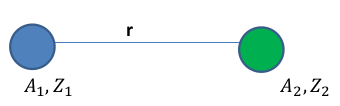
\includegraphics[scale=0.4]{ch8/image6}
	\captionof{figure}{ }
	\end{wrapfigure}
Supposons que le noyau soit formé de deux amas (\textit{cluster}) de nucléons à grande distance l'un de l'autre 
et que la structure interne de ces amas soit négligée.  L'Hamiltonien du noyau s'écrit
\begin{equation}
H=T_1+T_2 +V(r_1-r_2- = T_m-\frac{\hbar^2}{2\mu}\Delta_r+V(r)
\end{equation}
où $V(r)$ contient deux termes (un nucléaire et un coulombien) : $V(r)=V_N(r)+V_C(r)$.\\

A titre d'exemple, voici deux potentiels nucléaires contenant des paramètres ajustables
\begin{itemize}
\item[$\bullet$] Gaussien
\begin{equation}
V_N(r) = V_0\exp(-(r/r_0)^2)
\end{equation}
\item[$\bullet$] Woods-Saxon. Il contient un paramètre d'amplitude $V_0$, une portée $R$ et une diffusivité $a$. Il
a une forme "de marche" (alors que la gaussienne est plus arrondie : on parle de la partie gauche de la
gaussienne, prolongée ensuite par une droite). Pour $a=0$, il s'agit d'une marche anguleuse : la diffusivité
permet d'avoir une pente plus douce (elle vaut souvent 1/2 fermi).
\begin{equation}
V_N(r) = \frac{V_0}{1+\exp((r-R)/a)}
\end{equation}
\end{itemize}

\newpage
En considérant une fonction d'onde factorisée (un terme radial et un terme angulaire)
\begin{equation}
\Psi^{\ell m}(\vec{r}) = R_\ell(r)Y_\ell^m(\theta,\phi) = \frac{u_\ell(r)}{r}Y_\ell^m(\theta,\phi)
\end{equation}
On peut en obtenir l'équation radiale
\begin{equation}
-\frac{\hbar^2}{2\mu}\left(\frac{d^2}{dr^2}-\frac{\ell(\ell+1)}{r^2}\right)u_\ell + V(r)u_\ell + Eu_\ell
\end{equation}
Le comportement asymptotique pour $r$ petit (énergie positive ou négative) est donné par
\begin{equation}
u_\ell(r) \to r^{\ell+1}
\end{equation}
Le comportement asymptotique pour $r$ grand est donné par
\begin{equation}
\begin{array}{llll}
E > 0 &: u_\ell(r) &\to A\cos(kr)+B\sin(kr),&\qquad\text{avec } k=\sqrt{2\mu E/\hbar}\\
E < 0 &: u_\ell(r) &\to C\exp(-Kr),&\qquad\text{avec } K=\sqrt{-2\mu E/\hbar}
\end{array}
\end{equation}
Ici nous avons deux types de problème selon le signe de l'énergie (la physique diffère). Une énergie positive
représente la collision de deux noyaux où $E$ est alors l'énergie du faisceau. La solution est une onde plane.
L'énergie négative représente elle des états liés.\\

Il existe des potentiels simple où la solution analytique est connue (puits carré (deuton), oscillateur 
harmonique). Pour les deux exemples de potentiels repris ci-dessus, il n'existe pas de solution analytique
mais la résolution numérique est, elle, relativement aisée. Nous n'entrons ici pas dans les détails, le but était
de donner un aperçu de ce qui était faisable avec ce modèle.